\documentclass[1p]{elsarticle_modified}
%\bibliographystyle{elsarticle-num}

%\usepackage[colorlinks]{hyperref}
%\usepackage{abbrmath_seonhwa} %\Abb, \Ascr, \Acal ,\Abf, \Afrak
\usepackage{amsfonts}
\usepackage{amssymb}
\usepackage{amsmath}
\usepackage{amsthm}
\usepackage{scalefnt}
\usepackage{amsbsy}
\usepackage{kotex}
\usepackage{caption}
\usepackage{subfig}
\usepackage{color}
\usepackage{graphicx}
\usepackage{xcolor} %% white, black, red, green, blue, cyan, magenta, yellow
\usepackage{float}
\usepackage{setspace}
\usepackage{hyperref}

\usepackage{tikz}
\usetikzlibrary{arrows}

\usepackage{multirow}
\usepackage{array} % fixed length table
\usepackage{hhline}

%%%%%%%%%%%%%%%%%%%%%
\makeatletter
\renewcommand*\env@matrix[1][\arraystretch]{%
	\edef\arraystretch{#1}%
	\hskip -\arraycolsep
	\let\@ifnextchar\new@ifnextchar
	\array{*\c@MaxMatrixCols c}}
\makeatother %https://tex.stackexchange.com/questions/14071/how-can-i-increase-the-line-spacing-in-a-matrix
%%%%%%%%%%%%%%%

\usepackage[normalem]{ulem}

\newcommand{\msout}[1]{\ifmmode\text{\sout{\ensuremath{#1}}}\else\sout{#1}\fi}
%SOURCE: \msout is \stkout macro in https://tex.stackexchange.com/questions/20609/strikeout-in-math-mode

\newcommand{\cancel}[1]{
	\ifmmode
	{\color{red}\msout{#1}}
	\else
	{\color{red}\sout{#1}}
	\fi
}

\newcommand{\add}[1]{
	{\color{blue}\uwave{#1}}
}

\newcommand{\replace}[2]{
	\ifmmode
	{\color{red}\msout{#1}}{\color{blue}\uwave{#2}}
	\else
	{\color{red}\sout{#1}}{\color{blue}\uwave{#2}}
	\fi
}

\newcommand{\Sol}{\mathcal{S}} %segment
\newcommand{\D}{D} %diagram
\newcommand{\A}{\mathcal{A}} %arc


%%%%%%%%%%%%%%%%%%%%%%%%%%%%%5 test

\def\sl{\operatorname{\textup{SL}}(2,\Cbb)}
\def\psl{\operatorname{\textup{PSL}}(2,\Cbb)}
\def\quan{\mkern 1mu \triangleright \mkern 1mu}

\theoremstyle{definition}
\newtheorem{thm}{Theorem}[section]
\newtheorem{prop}[thm]{Proposition}
\newtheorem{lem}[thm]{Lemma}
\newtheorem{ques}[thm]{Question}
\newtheorem{cor}[thm]{Corollary}
\newtheorem{defn}[thm]{Definition}
\newtheorem{exam}[thm]{Example}
\newtheorem{rmk}[thm]{Remark}
\newtheorem{alg}[thm]{Algorithm}

\newcommand{\I}{\sqrt{-1}}
\begin{document}

%\begin{frontmatter}
%
%\title{Boundary parabolic representations of knots up to 8 crossings}
%
%%% Group authors per affiliation:
%\author{Yunhi Cho} 
%\address{Department of Mathematics, University of Seoul, Seoul, Korea}
%\ead{yhcho@uos.ac.kr}
%
%
%\author{Seonhwa Kim} %\fnref{s_kim}}
%\address{Center for Geometry and Physics, Institute for Basic Science, Pohang, 37673, Korea}
%\ead{ryeona17@ibs.re.kr}
%
%\author{Hyuk Kim}
%\address{Department of Mathematical Sciences, Seoul National University, Seoul 08826, Korea}
%\ead{hyukkim@snu.ac.kr}
%
%\author{Seokbeom Yoon}
%\address{Department of Mathematical Sciences, Seoul National University, Seoul, 08826,  Korea}
%\ead{sbyoon15@snu.ac.kr}
%
%\begin{abstract}
%We find all boundary parabolic representation of knots up to 8 crossings.
%
%\end{abstract}
%\begin{keyword}
%    \MSC[2010] 57M25 
%\end{keyword}
%
%\end{frontmatter}

%\linenumbers
%\tableofcontents
%
\newcommand\colored[1]{\textcolor{white}{\rule[-0.35ex]{0.8em}{1.4ex}}\kern-0.8em\color{red} #1}%
%\newcommand\colored[1]{\textcolor{white}{ #1}\kern-2.17ex	\textcolor{white}{ #1}\kern-1.81ex	\textcolor{white}{ #1}\kern-2.15ex\color{red}#1	}

{\Large $\underline{11a_{349}~(K11a_{349})}$}

\setlength{\tabcolsep}{10pt}
\renewcommand{\arraystretch}{1.6}
\vspace{1cm}\begin{tabular}{m{100pt}>{\centering\arraybackslash}m{274pt}}
\multirow{5}{120pt}{
	\centering
	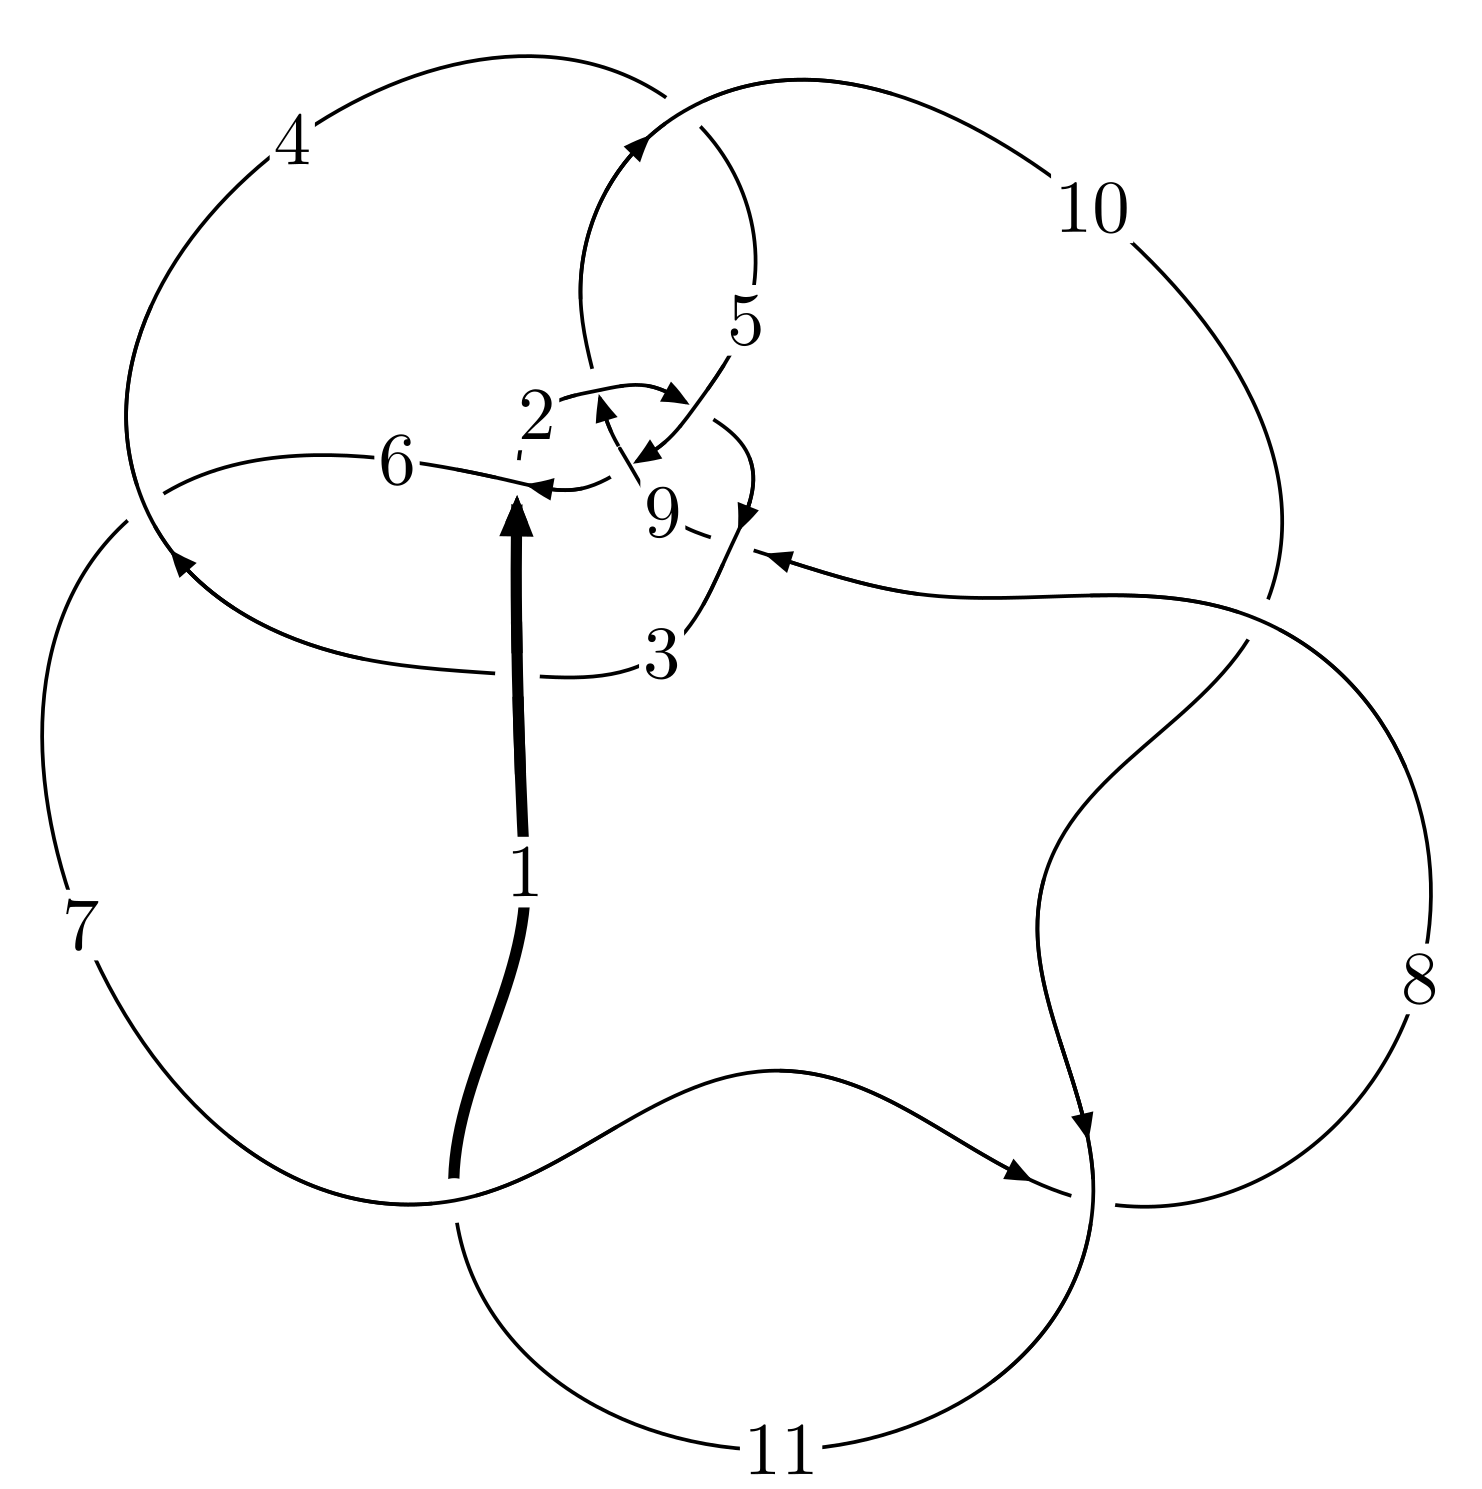
\includegraphics[width=112pt]{../../../GIT/diagram.site/Diagrams/png/598_11a_349.png}\\
\ \ \ A knot diagram\footnotemark}&
\allowdisplaybreaks
\textbf{Linearized knot diagam} \\
\cline{2-2}
 &
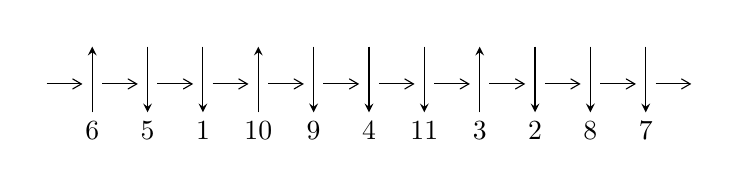
\begin{tikzpicture}[x=20pt, y=17pt]
	% nodes
	\node (C0) at (0, 0) {};
	\node (C1) at (1, 0) {};
	\node (C1U) at (1, +1) {};
	\node (C1D) at (1, -1) {6};

	\node (C2) at (2, 0) {};
	\node (C2U) at (2, +1) {};
	\node (C2D) at (2, -1) {5};

	\node (C3) at (3, 0) {};
	\node (C3U) at (3, +1) {};
	\node (C3D) at (3, -1) {1};

	\node (C4) at (4, 0) {};
	\node (C4U) at (4, +1) {};
	\node (C4D) at (4, -1) {10};

	\node (C5) at (5, 0) {};
	\node (C5U) at (5, +1) {};
	\node (C5D) at (5, -1) {9};

	\node (C6) at (6, 0) {};
	\node (C6U) at (6, +1) {};
	\node (C6D) at (6, -1) {4};

	\node (C7) at (7, 0) {};
	\node (C7U) at (7, +1) {};
	\node (C7D) at (7, -1) {11};

	\node (C8) at (8, 0) {};
	\node (C8U) at (8, +1) {};
	\node (C8D) at (8, -1) {3};

	\node (C9) at (9, 0) {};
	\node (C9U) at (9, +1) {};
	\node (C9D) at (9, -1) {2};

	\node (C10) at (10, 0) {};
	\node (C10U) at (10, +1) {};
	\node (C10D) at (10, -1) {8};

	\node (C11) at (11, 0) {};
	\node (C11U) at (11, +1) {};
	\node (C11D) at (11, -1) {7};
	\node (C12) at (12, 0) {};

	% arrows
	\draw[->,>={angle 60}]
	(C0) edge (C1) (C1) edge (C2) (C2) edge (C3) (C3) edge (C4) (C4) edge (C5) (C5) edge (C6) (C6) edge (C7) (C7) edge (C8) (C8) edge (C9) (C9) edge (C10) (C10) edge (C11) (C11) edge (C12) ;	\draw[->,>=stealth]
	(C1D) edge (C1U) (C2U) edge (C2D) (C3U) edge (C3D) (C4D) edge (C4U) (C5U) edge (C5D) (C6U) edge (C6D) (C7U) edge (C7D) (C8D) edge (C8U) (C9U) edge (C9D) (C10U) edge (C10D) (C11U) edge (C11D) ;
	\end{tikzpicture} \\
\hhline{~~} \\& 
\textbf{Solving Sequence} \\ \cline{2-2} 
 &
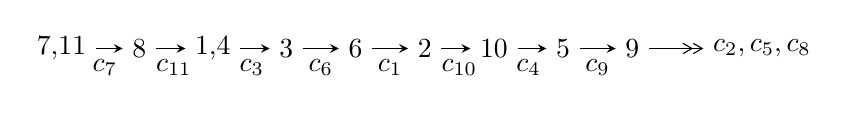
\begin{tikzpicture}[x=25pt, y=7pt]
	% node
	\node (A0) at (-1/8, 0) {7,11};
	\node (A1) at (1, 0) {8};
	\node (A2) at (33/16, 0) {1,4};
	\node (A3) at (25/8, 0) {3};
	\node (A4) at (33/8, 0) {6};
	\node (A5) at (41/8, 0) {2};
	\node (A6) at (49/8, 0) {10};
	\node (A7) at (57/8, 0) {5};
	\node (A8) at (65/8, 0) {9};
	\node (C1) at (1/2, -1) {$c_{7}$};
	\node (C2) at (3/2, -1) {$c_{11}$};
	\node (C3) at (21/8, -1) {$c_{3}$};
	\node (C4) at (29/8, -1) {$c_{6}$};
	\node (C5) at (37/8, -1) {$c_{1}$};
	\node (C6) at (45/8, -1) {$c_{10}$};
	\node (C7) at (53/8, -1) {$c_{4}$};
	\node (C8) at (61/8, -1) {$c_{9}$};
	\node (A9) at (10, 0) {$c_{2},c_{5},c_{8}$};

	% edge
	\draw[->,>=stealth]	
	(A0) edge (A1) (A1) edge (A2) (A2) edge (A3) (A3) edge (A4) (A4) edge (A5) (A5) edge (A6) (A6) edge (A7) (A7) edge (A8) ;
	\draw[->>,>={angle 60}]	
	(A8) edge (A9);
\end{tikzpicture} \\ 

\end{tabular} \\

\footnotetext{
The image of knot diagram is generated by the software ``\textbf{Draw programme}" developed by Andrew Bartholomew(\url{http://www.layer8.co.uk/maths/draw/index.htm\#Running-draw}), where we modified some parts for our purpose(\url{https://github.com/CATsTAILs/LinksPainter}).
}\phantom \\ \newline 
\centering \textbf{Ideals for irreducible components\footnotemark of $X_{\text{par}}$} 
 
\begin{align*}
I^u_{1}&=\langle 
-8794 u^{30}-59427 u^{29}+\cdots+14648 b-565817,\\
\phantom{I^u_{1}}&\phantom{= \langle  }1207779 u^{30}+10072486 u^{29}+\cdots+1069304 a-32922272,\;u^{31}+9 u^{30}+\cdots-608 u-73\rangle \\
I^u_{2}&=\langle 
1245599508 u^{14} a^3+2019297822 u^{14} a^2+\cdots+2559076525 a+1076862186,\\
\phantom{I^u_{2}}&\phantom{= \langle  }u^{14} a^2-3 u^{14}+\cdots- a+8,\\
\phantom{I^u_{2}}&\phantom{= \langle  }u^{15}-3 u^{14}+12 u^{13}-25 u^{12}+52 u^{11}-78 u^{10}+104 u^9-109 u^8+94 u^7-58 u^6+24 u^5+2 u^4-8 u^3+4 u^2-1\rangle \\
I^u_{3}&=\langle 
- u^{15}+5 u^{14}+\cdots+2 b+3 u,\;u^{15}-6 u^{14}+\cdots+2 a+3,\;u^{16}-4 u^{15}+\cdots+2 u^2+1\rangle \\
\\
I^v_{1}&=\langle 
a,\;b^2- b+1,\;v-1\rangle \\
\end{align*}
\raggedright * 4 irreducible components of $\dim_{\mathbb{C}}=0$, with total 109 representations.\\
\footnotetext{All coefficients of polynomials are rational numbers. But the coefficients are sometimes approximated in decimal forms when there is not enough margin.}
\newpage
\renewcommand{\arraystretch}{1}
\centering \section*{I. $I^u_{1}= \langle -8794 u^{30}-59427 u^{29}+\cdots+14648 b-565817,\;1.21\times10^{6} u^{30}+1.01\times10^{7} u^{29}+\cdots+1.07\times10^{6} a-3.29\times10^{7},\;u^{31}+9 u^{30}+\cdots-608 u-73 \rangle$}
\flushleft \textbf{(i) Arc colorings}\\
\begin{tabular}{m{7pt} m{180pt} m{7pt} m{180pt} }
\flushright $a_{7}=$&$\begin{pmatrix}1\\0\end{pmatrix}$ \\
\flushright $a_{11}=$&$\begin{pmatrix}0\\u\end{pmatrix}$ \\
\flushright $a_{8}=$&$\begin{pmatrix}1\\u^2\end{pmatrix}$ \\
\flushright $a_{1}=$&$\begin{pmatrix}- u\\u\end{pmatrix}$ \\
\flushright $a_{4}=$&$\begin{pmatrix}-1.12950 u^{30}-9.41967 u^{29}+\cdots+251.970 u+30.7885\\0.600355 u^{30}+4.05700 u^{29}+\cdots+252.304 u+38.6276\end{pmatrix}$ \\
\flushright $a_{3}=$&$\begin{pmatrix}0.216690 u^{30}+2.67536 u^{29}+\cdots-151.674 u-13.0374\\-0.745836 u^{30}-8.03803 u^{29}+\cdots+655.948 u+82.4535\end{pmatrix}$ \\
\flushright $a_{6}=$&$\begin{pmatrix}0.742167 u^{30}+6.23678 u^{29}+\cdots-18.8469 u+1.55985\\-0.689719 u^{30}-5.07503 u^{29}+\cdots-28.6196 u-3.82871\end{pmatrix}$ \\
\flushright $a_{2}=$&$\begin{pmatrix}-1.15640 u^{30}-8.25807 u^{29}+\cdots-113.632 u-15.8600\\-0.265838 u^{30}-5.40866 u^{29}+\cdots+1150.58 u+154.173\end{pmatrix}$ \\
\flushright $a_{10}=$&$\begin{pmatrix}u\\u^3+u\end{pmatrix}$ \\
\flushright $a_{5}=$&$\begin{pmatrix}-0.757026 u^{30}-7.25316 u^{29}+\cdots+294.147 u+32.3085\\1.10930 u^{30}+9.99788 u^{29}+\cdots-399.270 u-46.4128\end{pmatrix}$ \\
\flushright $a_{9}=$&$\begin{pmatrix}0.261828 u^{30}+1.90356 u^{29}+\cdots-25.4736 u-4.38300\\0.0106499 u^{30}+0.585131 u^{29}+\cdots-179.751 u-22.5472\end{pmatrix}$\\ \flushright $a_{9}=$&$\begin{pmatrix}0.261828 u^{30}+1.90356 u^{29}+\cdots-25.4736 u-4.38300\\0.0106499 u^{30}+0.585131 u^{29}+\cdots-179.751 u-22.5472\end{pmatrix}$\\&\end{tabular}
\flushleft \textbf{(ii) Obstruction class $= -1$}\\~\\
\flushleft \textbf{(iii) Cusp Shapes $= \frac{102043}{14648} u^{30}+\frac{113248}{1831} u^{29}+\cdots-\frac{59622049}{14648} u-\frac{4091199}{7324}$}\\~\\
\newpage\renewcommand{\arraystretch}{1}
\flushleft \textbf{(iv) u-Polynomials at the component}\newline \\
\begin{tabular}{m{50pt}|m{274pt}}
Crossings & \hspace{64pt}u-Polynomials at each crossing \\
\hline $$\begin{aligned}c_{1}\end{aligned}$$&$\begin{aligned}
&u^{31}-24 u^{30}+\cdots-360448 u+32768
\end{aligned}$\\
\hline $$\begin{aligned}c_{2}\end{aligned}$$&$\begin{aligned}
&u^{31}-22 u^{30}+\cdots+419 u-73
\end{aligned}$\\
\hline $$\begin{aligned}c_{3},c_{6}\end{aligned}$$&$\begin{aligned}
&u^{31}+u^{30}+\cdots+14 u+1
\end{aligned}$\\
\hline $$\begin{aligned}c_{4},c_{8}\end{aligned}$$&$\begin{aligned}
&u^{31}- u^{30}+\cdots-2 u+1
\end{aligned}$\\
\hline $$\begin{aligned}c_{5},c_{9}\end{aligned}$$&$\begin{aligned}
&u^{31}+u^{29}+\cdots+2 u+1
\end{aligned}$\\
\hline $$\begin{aligned}c_{7},c_{10},c_{11}\end{aligned}$$&$\begin{aligned}
&u^{31}-9 u^{30}+\cdots-608 u+73
\end{aligned}$\\
\hline
\end{tabular}\\~\\
\newpage\renewcommand{\arraystretch}{1}
\flushleft \textbf{(v) Riley Polynomials at the component}\newline \\
\begin{tabular}{m{50pt}|m{274pt}}
Crossings & \hspace{64pt}Riley Polynomials at each crossing \\
\hline $$\begin{aligned}c_{1}\end{aligned}$$&$\begin{aligned}
&y^{31}+10 y^{30}+\cdots-2147483648 y-1073741824
\end{aligned}$\\
\hline $$\begin{aligned}c_{2}\end{aligned}$$&$\begin{aligned}
&y^{31}+46 y^{29}+\cdots+42263 y-5329
\end{aligned}$\\
\hline $$\begin{aligned}c_{3},c_{6}\end{aligned}$$&$\begin{aligned}
&y^{31}+15 y^{30}+\cdots+110 y-1
\end{aligned}$\\
\hline $$\begin{aligned}c_{4},c_{8}\end{aligned}$$&$\begin{aligned}
&y^{31}+7 y^{30}+\cdots-40 y-1
\end{aligned}$\\
\hline $$\begin{aligned}c_{5},c_{9}\end{aligned}$$&$\begin{aligned}
&y^{31}+2 y^{30}+\cdots-6 y-1
\end{aligned}$\\
\hline $$\begin{aligned}c_{7},c_{10},c_{11}\end{aligned}$$&$\begin{aligned}
&y^{31}+31 y^{30}+\cdots-37092 y-5329
\end{aligned}$\\
\hline
\end{tabular}\\~\\
\newpage\flushleft \textbf{(vi) Complex Volumes and Cusp Shapes}
$$\begin{array}{c|c|c}  
\text{Solutions to }I^u_{1}& \I (\text{vol} + \sqrt{-1}CS) & \text{Cusp shape}\\
 \hline 
\begin{aligned}
u &= -0.852991 + 0.499323 I \\
a &= -0.379018 - 0.633422 I \\
b &= -0.994010 + 0.988244 I\end{aligned}
 & -3.36735 + 13.70180 I & -6.58812 - 9.58074 I \\ \hline\begin{aligned}
u &= -0.852991 - 0.499323 I \\
a &= -0.379018 + 0.633422 I \\
b &= -0.994010 - 0.988244 I\end{aligned}
 & -3.36735 - 13.70180 I & -6.58812 + 9.58074 I \\ \hline\begin{aligned}
u &= -0.316579 + 0.888214 I \\
a &= -1.097970 + 0.312101 I \\
b &= \phantom{-}0.721245 + 0.634191 I\end{aligned}
 & -0.90699 - 1.43155 I & -3.87159 + 9.73821 I \\ \hline\begin{aligned}
u &= -0.316579 - 0.888214 I \\
a &= -1.097970 - 0.312101 I \\
b &= \phantom{-}0.721245 - 0.634191 I\end{aligned}
 & -0.90699 + 1.43155 I & -3.87159 - 9.73821 I \\ \hline\begin{aligned}
u &= -0.886962 + 0.303700 I \\
a &= \phantom{-}0.332501 + 0.072745 I \\
b &= \phantom{-}0.235798 - 0.956055 I\end{aligned}
 & \phantom{-}1.08264 + 5.12278 I & -0.41195 - 8.68112 I \\ \hline\begin{aligned}
u &= -0.886962 - 0.303700 I \\
a &= \phantom{-}0.332501 - 0.072745 I \\
b &= \phantom{-}0.235798 + 0.956055 I\end{aligned}
 & \phantom{-}1.08264 - 5.12278 I & -0.41195 + 8.68112 I \\ \hline\begin{aligned}
u &= -0.844232 + 0.691840 I \\
a &= \phantom{-}0.578588 - 0.200674 I \\
b &= -0.675443 - 0.657436 I\end{aligned}
 & -2.87005 - 8.08181 I & -6.17763 + 7.71756 I \\ \hline\begin{aligned}
u &= -0.844232 - 0.691840 I \\
a &= \phantom{-}0.578588 + 0.200674 I \\
b &= -0.675443 + 0.657436 I\end{aligned}
 & -2.87005 + 8.08181 I & -6.17763 - 7.71756 I \\ \hline\begin{aligned}
u &= \phantom{-}1.18811\phantom{ +0.000000I} \\
a &= -0.163592\phantom{ +0.000000I} \\
b &= \phantom{-}0.0888281\phantom{ +0.000000I}\end{aligned}
 & -2.36361\phantom{ +0.000000I} & \phantom{-}35.4320\phantom{ +0.000000I} \\ \hline\begin{aligned}
u &= -0.722698 + 0.301514 I \\
a &= \phantom{-}0.681450 + 0.287166 I \\
b &= \phantom{-}0.960625 - 1.037040 I\end{aligned}
 & -2.64536 + 5.39096 I & -12.5250 - 11.7577 I\\
 \hline 
 \end{array}$$\newpage$$\begin{array}{c|c|c}  
\text{Solutions to }I^u_{1}& \I (\text{vol} + \sqrt{-1}CS) & \text{Cusp shape}\\
 \hline 
\begin{aligned}
u &= -0.722698 - 0.301514 I \\
a &= \phantom{-}0.681450 - 0.287166 I \\
b &= \phantom{-}0.960625 + 1.037040 I\end{aligned}
 & -2.64536 - 5.39096 I & -12.5250 + 11.7577 I \\ \hline\begin{aligned}
u &= -0.403264 + 0.649558 I \\
a &= -0.871610 - 0.575987 I \\
b &= -0.277793 + 0.861904 I\end{aligned}
 & \phantom{-}2.96693 - 0.69018 I & \phantom{-}2.10294 + 0.24214 I \\ \hline\begin{aligned}
u &= -0.403264 - 0.649558 I \\
a &= -0.871610 + 0.575987 I \\
b &= -0.277793 - 0.861904 I\end{aligned}
 & \phantom{-}2.96693 + 0.69018 I & \phantom{-}2.10294 - 0.24214 I \\ \hline\begin{aligned}
u &= -0.281651 + 1.296450 I \\
a &= -0.574322 - 0.910235 I \\
b &= -0.150654 + 0.951529 I\end{aligned}
 & \phantom{-}3.76674 - 0.82301 I & \phantom{-0.000000 } 0 \\ \hline\begin{aligned}
u &= -0.281651 - 1.296450 I \\
a &= -0.574322 + 0.910235 I \\
b &= -0.150654 - 0.951529 I\end{aligned}
 & \phantom{-}3.76674 + 0.82301 I & \phantom{-0.000000 } 0 \\ \hline\begin{aligned}
u &= \phantom{-}0.013670 + 1.401210 I \\
a &= -0.09185 + 1.89114 I \\
b &= \phantom{-}0.94670 - 1.20717 I\end{aligned}
 & \phantom{-}4.82828 + 1.90483 I & \phantom{-0.000000 } 0 \\ \hline\begin{aligned}
u &= \phantom{-}0.013670 - 1.401210 I \\
a &= -0.09185 - 1.89114 I \\
b &= \phantom{-}0.94670 + 1.20717 I\end{aligned}
 & \phantom{-}4.82828 - 1.90483 I & \phantom{-0.000000 } 0 \\ \hline\begin{aligned}
u &= \phantom{-}0.297730 + 0.511306 I \\
a &= -0.978614 - 0.248724 I \\
b &= \phantom{-}0.260483 + 0.340007 I\end{aligned}
 & -0.38522 - 1.41061 I & -2.90382 + 5.08297 I \\ \hline\begin{aligned}
u &= \phantom{-}0.297730 - 0.511306 I \\
a &= -0.978614 + 0.248724 I \\
b &= \phantom{-}0.260483 - 0.340007 I\end{aligned}
 & -0.38522 + 1.41061 I & -2.90382 - 5.08297 I \\ \hline\begin{aligned}
u &= \phantom{-}0.06166 + 1.42151 I \\
a &= -0.130706 - 1.235920 I \\
b &= -0.471500 + 0.878105 I\end{aligned}
 & \phantom{-}5.49366 - 2.37184 I & \phantom{-0.000000 } 0\\
 \hline 
 \end{array}$$\newpage$$\begin{array}{c|c|c}  
\text{Solutions to }I^u_{1}& \I (\text{vol} + \sqrt{-1}CS) & \text{Cusp shape}\\
 \hline 
\begin{aligned}
u &= \phantom{-}0.06166 - 1.42151 I \\
a &= -0.130706 + 1.235920 I \\
b &= -0.471500 - 0.878105 I\end{aligned}
 & \phantom{-}5.49366 + 2.37184 I & \phantom{-0.000000 } 0 \\ \hline\begin{aligned}
u &= -0.26782 + 1.43933 I \\
a &= -0.00779 + 1.93679 I \\
b &= \phantom{-}1.07459 - 1.38869 I\end{aligned}
 & \phantom{-}2.96780 + 8.97601 I & \phantom{-0.000000 } 0 \\ \hline\begin{aligned}
u &= -0.26782 - 1.43933 I \\
a &= -0.00779 - 1.93679 I \\
b &= \phantom{-}1.07459 + 1.38869 I\end{aligned}
 & \phantom{-}2.96780 - 8.97601 I & \phantom{-0.000000 } 0 \\ \hline\begin{aligned}
u &= -0.14638 + 1.50740 I \\
a &= -0.13509 - 1.58317 I \\
b &= -0.698585 + 1.200690 I\end{aligned}
 & \phantom{-}9.90733 + 1.39993 I & \phantom{-0.000000 } 0 \\ \hline\begin{aligned}
u &= -0.14638 - 1.50740 I \\
a &= -0.13509 + 1.58317 I \\
b &= -0.698585 - 1.200690 I\end{aligned}
 & \phantom{-}9.90733 - 1.39993 I & \phantom{-0.000000 } 0 \\ \hline\begin{aligned}
u &= -0.33955 + 1.47960 I \\
a &= \phantom{-}0.39739 + 1.41421 I \\
b &= \phantom{-}0.499587 - 1.282410 I\end{aligned}
 & \phantom{-}6.87874 + 9.56615 I & \phantom{-0.000000 } 0 \\ \hline\begin{aligned}
u &= -0.33955 - 1.47960 I \\
a &= \phantom{-}0.39739 - 1.41421 I \\
b &= \phantom{-}0.499587 + 1.282410 I\end{aligned}
 & \phantom{-}6.87874 - 9.56615 I & \phantom{-0.000000 } 0 \\ \hline\begin{aligned}
u &= -0.30764 + 1.52681 I \\
a &= \phantom{-}0.13457 - 1.85476 I \\
b &= -1.10902 + 1.32474 I\end{aligned}
 & \phantom{-}3.1915 + 17.9314 I & \phantom{-0.000000 } 0 \\ \hline\begin{aligned}
u &= -0.30764 - 1.52681 I \\
a &= \phantom{-}0.13457 + 1.85476 I \\
b &= -1.10902 - 1.32474 I\end{aligned}
 & \phantom{-}3.1915 - 17.9314 I & \phantom{-0.000000 } 0 \\ \hline\begin{aligned}
u &= -0.09735 + 1.67029 I \\
a &= \phantom{-}0.203729 + 0.617797 I \\
b &= \phantom{-}0.133556 - 0.557496 I\end{aligned}
 & \phantom{-}5.63925 - 4.20521 I & \phantom{-0.000000 } 0\\
 \hline 
 \end{array}$$\newpage$$\begin{array}{c|c|c}  
\text{Solutions to }I^u_{1}& \I (\text{vol} + \sqrt{-1}CS) & \text{Cusp shape}\\
 \hline 
\begin{aligned}
u &= -0.09735 - 1.67029 I \\
a &= \phantom{-}0.203729 - 0.617797 I \\
b &= \phantom{-}0.133556 + 0.557496 I\end{aligned}
 & \phantom{-}5.63925 + 4.20521 I & \phantom{-0.000000 } 0\\
 \hline 
 \end{array}$$\newpage\newpage\renewcommand{\arraystretch}{1}
\centering \section*{II. $I^u_{2}= \langle 1.25\times10^{9} a^{3} u^{14}+2.02\times10^{9} a^{2} u^{14}+\cdots+2.56\times10^{9} a+1.08\times10^{9},\;u^{14} a^2-3 u^{14}+\cdots- a+8,\;u^{15}-3 u^{14}+\cdots+4 u^2-1 \rangle$}
\flushleft \textbf{(i) Arc colorings}\\
\begin{tabular}{m{7pt} m{180pt} m{7pt} m{180pt} }
\flushright $a_{7}=$&$\begin{pmatrix}1\\0\end{pmatrix}$ \\
\flushright $a_{11}=$&$\begin{pmatrix}0\\u\end{pmatrix}$ \\
\flushright $a_{8}=$&$\begin{pmatrix}1\\u^2\end{pmatrix}$ \\
\flushright $a_{1}=$&$\begin{pmatrix}- u\\u\end{pmatrix}$ \\
\flushright $a_{4}=$&$\begin{pmatrix}a\\-0.817912 a^{3} u^{14}-1.32595 a^{2} u^{14}+\cdots-1.68039 a-0.707112\end{pmatrix}$ \\
\flushright $a_{3}=$&$\begin{pmatrix}-0.471824 a^{3} u^{14}+0.346733 a^{2} u^{14}+\cdots+0.195001 a-0.931134\\-0.346088 a^{3} u^{14}-1.67269 a^{2} u^{14}+\cdots-0.875395 a+0.224022\end{pmatrix}$ \\
\flushright $a_{6}=$&$\begin{pmatrix}-0.0699739 a^{3} u^{14}-0.319988 a^{2} u^{14}+\cdots+0.0210967 a+0.491055\\-0.0602705 a^{3} u^{14}-0.0972240 a^{2} u^{14}+\cdots-0.701805 a+0.161294\end{pmatrix}$ \\
\flushright $a_{2}=$&$\begin{pmatrix}-0.548073 a^{3} u^{14}-0.225684 a^{2} u^{14}+\cdots-0.0705041 a+0.0289120\\0.417828 a^{3} u^{14}-0.191528 a^{2} u^{14}+\cdots-0.610204 a+0.623437\end{pmatrix}$ \\
\flushright $a_{10}=$&$\begin{pmatrix}u\\u^3+u\end{pmatrix}$ \\
\flushright $a_{5}=$&$\begin{pmatrix}-0.471824 a^{3} u^{14}+0.346733 a^{2} u^{14}+\cdots+0.195001 a-0.931134\\-1.19479 a^{3} u^{14}-1.41931 a^{2} u^{14}+\cdots-1.33430 a-0.154021\end{pmatrix}$ \\
\flushright $a_{9}=$&$\begin{pmatrix}-0.923492 a^{3} u^{14}+0.378846 a^{2} u^{14}+\cdots-0.912625 a-0.744597\\0.765493 a^{3} u^{14}-1.51930 a^{2} u^{14}+\cdots-0.488395 a+1.38890\end{pmatrix}$\\ \flushright $a_{9}=$&$\begin{pmatrix}-0.923492 a^{3} u^{14}+0.378846 a^{2} u^{14}+\cdots-0.912625 a-0.744597\\0.765493 a^{3} u^{14}-1.51930 a^{2} u^{14}+\cdots-0.488395 a+1.38890\end{pmatrix}$\\&\end{tabular}
\flushleft \textbf{(ii) Obstruction class $= -1$}\\~\\
\flushleft \textbf{(iii) Cusp Shapes $= \frac{271921296}{138445675} u^{14} a^3+\frac{88680364}{138445675} u^{14} a^2+\cdots+\frac{17490488}{5537827} a-\frac{1797460618}{138445675}$}\\~\\
\newpage\renewcommand{\arraystretch}{1}
\flushleft \textbf{(iv) u-Polynomials at the component}\newline \\
\begin{tabular}{m{50pt}|m{274pt}}
Crossings & \hspace{64pt}u-Polynomials at each crossing \\
\hline $$\begin{aligned}c_{1}\end{aligned}$$&$\begin{aligned}
&(u^2+u+1)^{30}
\end{aligned}$\\
\hline $$\begin{aligned}c_{2}\end{aligned}$$&$\begin{aligned}
&(u^{15}+7 u^{14}+\cdots-4 u^2+1)^{4}
\end{aligned}$\\
\hline $$\begin{aligned}c_{3},c_{6}\end{aligned}$$&$\begin{aligned}
&u^{60}+u^{59}+\cdots+12 u+7
\end{aligned}$\\
\hline $$\begin{aligned}c_{4},c_{8}\end{aligned}$$&$\begin{aligned}
&u^{60}- u^{59}+\cdots-19478 u+3673
\end{aligned}$\\
\hline $$\begin{aligned}c_{5},c_{9}\end{aligned}$$&$\begin{aligned}
&u^{60}- u^{59}+\cdots+6 u+1
\end{aligned}$\\
\hline $$\begin{aligned}c_{7},c_{10},c_{11}\end{aligned}$$&$\begin{aligned}
&(u^{15}+3 u^{14}+\cdots-4 u^2+1)^{4}
\end{aligned}$\\
\hline
\end{tabular}\\~\\
\newpage\renewcommand{\arraystretch}{1}
\flushleft \textbf{(v) Riley Polynomials at the component}\newline \\
\begin{tabular}{m{50pt}|m{274pt}}
Crossings & \hspace{64pt}Riley Polynomials at each crossing \\
\hline $$\begin{aligned}c_{1}\end{aligned}$$&$\begin{aligned}
&(y^2+y+1)^{30}
\end{aligned}$\\
\hline $$\begin{aligned}c_{2}\end{aligned}$$&$\begin{aligned}
&(y^{15}- y^{14}+\cdots+8 y-1)^{4}
\end{aligned}$\\
\hline $$\begin{aligned}c_{3},c_{6}\end{aligned}$$&$\begin{aligned}
&y^{60}-9 y^{59}+\cdots-256 y+49
\end{aligned}$\\
\hline $$\begin{aligned}c_{4},c_{8}\end{aligned}$$&$\begin{aligned}
&y^{60}+15 y^{59}+\cdots+261046488 y+13490929
\end{aligned}$\\
\hline $$\begin{aligned}c_{5},c_{9}\end{aligned}$$&$\begin{aligned}
&y^{60}-21 y^{59}+\cdots-228 y^2+1
\end{aligned}$\\
\hline $$\begin{aligned}c_{7},c_{10},c_{11}\end{aligned}$$&$\begin{aligned}
&(y^{15}+15 y^{14}+\cdots+8 y-1)^{4}
\end{aligned}$\\
\hline
\end{tabular}\\~\\
\newpage\flushleft \textbf{(vi) Complex Volumes and Cusp Shapes}
$$\begin{array}{c|c|c}  
\text{Solutions to }I^u_{2}& \I (\text{vol} + \sqrt{-1}CS) & \text{Cusp shape}\\
 \hline 
\begin{aligned}
u &= \phantom{-}0.825834 + 0.538674 I \\
a &= \phantom{-}0.179032 - 0.898220 I \\
b &= \phantom{-}0.942665 + 0.900730 I\end{aligned}
 & -2.77564 - 4.75250 I & -17.6934 + 11.6845 I \\ \hline\begin{aligned}
u &= \phantom{-}0.825834 + 0.538674 I \\
a &= \phantom{-}0.064202 + 0.531611 I \\
b &= -0.515882 + 0.190551 I\end{aligned}
 & -2.77564 - 0.69273 I & -17.6934 + 4.7563 I \\ \hline\begin{aligned}
u &= \phantom{-}0.825834 + 0.538674 I \\
a &= -0.374874 + 0.363480 I \\
b &= -0.924983 - 0.606302 I\end{aligned}
 & -2.77564 - 4.75250 I & -17.6934 + 11.6845 I \\ \hline\begin{aligned}
u &= \phantom{-}0.825834 + 0.538674 I \\
a &= -0.429379 - 0.094637 I \\
b &= \phantom{-}0.762023 - 0.353078 I\end{aligned}
 & -2.77564 - 0.69273 I & -17.6934 + 4.7563 I \\ \hline\begin{aligned}
u &= \phantom{-}0.825834 - 0.538674 I \\
a &= \phantom{-}0.179032 + 0.898220 I \\
b &= \phantom{-}0.942665 - 0.900730 I\end{aligned}
 & -2.77564 + 4.75250 I & -17.6934 - 11.6845 I \\ \hline\begin{aligned}
u &= \phantom{-}0.825834 - 0.538674 I \\
a &= \phantom{-}0.064202 - 0.531611 I \\
b &= -0.515882 - 0.190551 I\end{aligned}
 & -2.77564 + 0.69273 I & -17.6934 - 4.7563 I \\ \hline\begin{aligned}
u &= \phantom{-}0.825834 - 0.538674 I \\
a &= -0.374874 - 0.363480 I \\
b &= -0.924983 + 0.606302 I\end{aligned}
 & -2.77564 + 4.75250 I & -17.6934 - 11.6845 I \\ \hline\begin{aligned}
u &= \phantom{-}0.825834 - 0.538674 I \\
a &= -0.429379 + 0.094637 I \\
b &= \phantom{-}0.762023 + 0.353078 I\end{aligned}
 & -2.77564 + 0.69273 I & -17.6934 - 4.7563 I \\ \hline\begin{aligned}
u &= -0.000696 + 1.255430 I \\
a &= -0.537288 + 0.318620 I \\
b &= -1.054520 - 0.277320 I\end{aligned}
 & \phantom{-}0.17890 - 4.56727 I & -8.44510 + 5.18626 I \\ \hline\begin{aligned}
u &= -0.000696 + 1.255430 I \\
a &= -1.53790 - 0.07369 I \\
b &= \phantom{-}1.74600 + 0.26986 I\end{aligned}
 & \phantom{-}0.178899 - 0.507500 I & -8.44510 - 1.74195 I\\
 \hline 
 \end{array}$$\newpage$$\begin{array}{c|c|c}  
\text{Solutions to }I^u_{2}& \I (\text{vol} + \sqrt{-1}CS) & \text{Cusp shape}\\
 \hline 
\begin{aligned}
u &= -0.000696 + 1.255430 I \\
a &= -0.46059 + 1.65199 I \\
b &= \phantom{-}0.246412 - 0.261109 I\end{aligned}
 & \phantom{-}0.178899 - 0.507500 I & -8.44510 - 1.74195 I \\ \hline\begin{aligned}
u &= -0.000696 + 1.255430 I \\
a &= \phantom{-}0.16969 - 2.83852 I \\
b &= \phantom{-}0.05074 + 1.99842 I\end{aligned}
 & \phantom{-}0.17890 - 4.56727 I & -8.44510 + 5.18626 I \\ \hline\begin{aligned}
u &= -0.000696 - 1.255430 I \\
a &= -0.537288 - 0.318620 I \\
b &= -1.054520 + 0.277320 I\end{aligned}
 & \phantom{-}0.17890 + 4.56727 I & -8.44510 - 5.18626 I \\ \hline\begin{aligned}
u &= -0.000696 - 1.255430 I \\
a &= -1.53790 + 0.07369 I \\
b &= \phantom{-}1.74600 - 0.26986 I\end{aligned}
 & \phantom{-}0.178899 + 0.507500 I & -8.44510 + 1.74195 I \\ \hline\begin{aligned}
u &= -0.000696 - 1.255430 I \\
a &= -0.46059 - 1.65199 I \\
b &= \phantom{-}0.246412 + 0.261109 I\end{aligned}
 & \phantom{-}0.178899 + 0.507500 I & -8.44510 + 1.74195 I \\ \hline\begin{aligned}
u &= -0.000696 - 1.255430 I \\
a &= \phantom{-}0.16969 + 2.83852 I \\
b &= \phantom{-}0.05074 - 1.99842 I\end{aligned}
 & \phantom{-}0.17890 + 4.56727 I & -8.44510 - 5.18626 I \\ \hline\begin{aligned}
u &= \phantom{-}0.374558 + 0.641779 I \\
a &= -1.242750 - 0.072310 I \\
b &= \phantom{-}0.404571 - 0.052904 I\end{aligned}
 & -0.331160 - 1.366830 I & -2.47200 + 4.73263 I \\ \hline\begin{aligned}
u &= \phantom{-}0.374558 + 0.641779 I \\
a &= -0.211923 + 0.547582 I \\
b &= -1.227140 - 0.690327 I\end{aligned}
 & -0.33116 - 5.42660 I & -2.47200 + 11.66083 I \\ \hline\begin{aligned}
u &= \phantom{-}0.374558 + 0.641779 I \\
a &= -0.446534 - 0.078718 I \\
b &= \phantom{-}0.233588 + 0.584828 I\end{aligned}
 & -0.331160 - 1.366830 I & -2.47200 + 4.73263 I \\ \hline\begin{aligned}
u &= \phantom{-}0.374558 + 0.641779 I \\
a &= \phantom{-}1.18736 - 1.93503 I \\
b &= \phantom{-}0.447402 + 0.977027 I\end{aligned}
 & -0.33116 - 5.42660 I & -2.47200 + 11.66083 I\\
 \hline 
 \end{array}$$\newpage$$\begin{array}{c|c|c}  
\text{Solutions to }I^u_{2}& \I (\text{vol} + \sqrt{-1}CS) & \text{Cusp shape}\\
 \hline 
\begin{aligned}
u &= \phantom{-}0.374558 - 0.641779 I \\
a &= -1.242750 + 0.072310 I \\
b &= \phantom{-}0.404571 + 0.052904 I\end{aligned}
 & -0.331160 + 1.366830 I & -2.47200 - 4.73263 I \\ \hline\begin{aligned}
u &= \phantom{-}0.374558 - 0.641779 I \\
a &= -0.211923 - 0.547582 I \\
b &= -1.227140 + 0.690327 I\end{aligned}
 & -0.33116 + 5.42660 I & -2.47200 - 11.66083 I \\ \hline\begin{aligned}
u &= \phantom{-}0.374558 - 0.641779 I \\
a &= -0.446534 + 0.078718 I \\
b &= \phantom{-}0.233588 - 0.584828 I\end{aligned}
 & -0.331160 + 1.366830 I & -2.47200 - 4.73263 I \\ \hline\begin{aligned}
u &= \phantom{-}0.374558 - 0.641779 I \\
a &= \phantom{-}1.18736 + 1.93503 I \\
b &= \phantom{-}0.447402 - 0.977027 I\end{aligned}
 & -0.33116 + 5.42660 I & -2.47200 - 11.66083 I \\ \hline\begin{aligned}
u &= \phantom{-}0.678314\phantom{ +0.000000I} \\
a &= -0.755171 + 1.008870 I \\
b &= -0.575180 + 0.365490 I\end{aligned}
 & -2.66135 + 2.02988 I & -15.2719 - 3.4641 I \\ \hline\begin{aligned}
u &= \phantom{-}0.678314\phantom{ +0.000000I} \\
a &= -0.755171 - 1.008870 I \\
b &= -0.575180 - 0.365490 I\end{aligned}
 & -2.66135 - 2.02988 I & -15.2719 + 3.4641 I \\ \hline\begin{aligned}
u &= \phantom{-}0.678314\phantom{ +0.000000I} \\
a &= -0.054442 + 0.393425 I \\
b &= \phantom{-}0.902396 - 0.932245 I\end{aligned}
 & -2.66135 + 2.02988 I & -15.2719 - 3.4641 I \\ \hline\begin{aligned}
u &= \phantom{-}0.678314\phantom{ +0.000000I} \\
a &= -0.054442 - 0.393425 I \\
b &= \phantom{-}0.902396 + 0.932245 I\end{aligned}
 & -2.66135 - 2.02988 I & -15.2719 + 3.4641 I \\ \hline\begin{aligned}
u &= -0.100337 + 1.375660 I \\
a &= -0.339092 + 0.510735 I \\
b &= \phantom{-}1.44399 - 0.16542 I\end{aligned}
 & \phantom{-}1.67680 + 3.56562 I & -5.33049 - 4.32935 I \\ \hline\begin{aligned}
u &= -0.100337 + 1.375660 I \\
a &= \phantom{-}0.86553 - 2.02688 I \\
b &= -0.113467 + 0.277530 I\end{aligned}
 & \phantom{-}1.67680 + 7.62538 I & -5.33049 - 11.25756 I\\
 \hline 
 \end{array}$$\newpage$$\begin{array}{c|c|c}  
\text{Solutions to }I^u_{2}& \I (\text{vol} + \sqrt{-1}CS) & \text{Cusp shape}\\
 \hline 
\begin{aligned}
u &= -0.100337 + 1.375660 I \\
a &= \phantom{-}2.12438 + 1.14269 I \\
b &= -2.33104 - 1.21010 I\end{aligned}
 & \phantom{-}1.67680 + 7.62538 I & -5.33049 - 11.25756 I \\ \hline\begin{aligned}
u &= -0.100337 + 1.375660 I \\
a &= -0.39013 + 2.52070 I \\
b &= \phantom{-}0.58590 - 1.48531 I\end{aligned}
 & \phantom{-}1.67680 + 3.56562 I & -5.33049 - 4.32935 I \\ \hline\begin{aligned}
u &= -0.100337 - 1.375660 I \\
a &= -0.339092 - 0.510735 I \\
b &= \phantom{-}1.44399 + 0.16542 I\end{aligned}
 & \phantom{-}1.67680 - 3.56562 I & -5.33049 + 4.32935 I \\ \hline\begin{aligned}
u &= -0.100337 - 1.375660 I \\
a &= \phantom{-}0.86553 + 2.02688 I \\
b &= -0.113467 - 0.277530 I\end{aligned}
 & \phantom{-}1.67680 - 7.62538 I & -5.33049 + 11.25756 I \\ \hline\begin{aligned}
u &= -0.100337 - 1.375660 I \\
a &= \phantom{-}2.12438 - 1.14269 I \\
b &= -2.33104 + 1.21010 I\end{aligned}
 & \phantom{-}1.67680 - 7.62538 I & -5.33049 + 11.25756 I \\ \hline\begin{aligned}
u &= -0.100337 - 1.375660 I \\
a &= -0.39013 - 2.52070 I \\
b &= \phantom{-}0.58590 + 1.48531 I\end{aligned}
 & \phantom{-}1.67680 - 3.56562 I & -5.33049 + 4.32935 I \\ \hline\begin{aligned}
u &= \phantom{-}0.15235 + 1.51729 I \\
a &= -0.521531 + 0.526784 I \\
b &= -0.380642 - 0.366400 I\end{aligned}
 & \phantom{-}6.67569 - 3.44689 I & \phantom{-}2.29813 + 1.92370 I \\ \hline\begin{aligned}
u &= \phantom{-}0.15235 + 1.51729 I \\
a &= -0.11679 - 1.56879 I \\
b &= \phantom{-}0.380795 + 1.344430 I\end{aligned}
 & \phantom{-}6.67569 - 3.44689 I & \phantom{-}2.29813 + 1.92370 I \\ \hline\begin{aligned}
u &= \phantom{-}0.15235 + 1.51729 I \\
a &= \phantom{-}0.36895 - 1.83783 I \\
b &= \phantom{-}0.665586 + 0.944764 I\end{aligned}
 & \phantom{-}6.67569 - 7.50666 I & \phantom{-}2.29813 + 8.85191 I \\ \hline\begin{aligned}
u &= \phantom{-}0.15235 + 1.51729 I \\
a &= \phantom{-}0.85260 + 1.80604 I \\
b &= -1.51266 - 1.43364 I\end{aligned}
 & \phantom{-}6.67569 - 7.50666 I & \phantom{-}2.29813 + 8.85191 I\\
 \hline 
 \end{array}$$\newpage$$\begin{array}{c|c|c}  
\text{Solutions to }I^u_{2}& \I (\text{vol} + \sqrt{-1}CS) & \text{Cusp shape}\\
 \hline 
\begin{aligned}
u &= \phantom{-}0.15235 - 1.51729 I \\
a &= -0.521531 - 0.526784 I \\
b &= -0.380642 + 0.366400 I\end{aligned}
 & \phantom{-}6.67569 + 3.44689 I & \phantom{-}2.29813 - 1.92370 I \\ \hline\begin{aligned}
u &= \phantom{-}0.15235 - 1.51729 I \\
a &= -0.11679 + 1.56879 I \\
b &= \phantom{-}0.380795 - 1.344430 I\end{aligned}
 & \phantom{-}6.67569 + 3.44689 I & \phantom{-}2.29813 - 1.92370 I \\ \hline\begin{aligned}
u &= \phantom{-}0.15235 - 1.51729 I \\
a &= \phantom{-}0.36895 + 1.83783 I \\
b &= \phantom{-}0.665586 - 0.944764 I\end{aligned}
 & \phantom{-}6.67569 + 7.50666 I & \phantom{-}2.29813 - 8.85191 I \\ \hline\begin{aligned}
u &= \phantom{-}0.15235 - 1.51729 I \\
a &= \phantom{-}0.85260 - 1.80604 I \\
b &= -1.51266 + 1.43364 I\end{aligned}
 & \phantom{-}6.67569 + 7.50666 I & \phantom{-}2.29813 - 8.85191 I \\ \hline\begin{aligned}
u &= \phantom{-}0.29798 + 1.53037 I \\
a &= -0.206885 + 1.025480 I \\
b &= -0.293963 - 0.641758 I\end{aligned}
 & \phantom{-}3.91480 - 4.81769 I & -7.00546 + 6.81035 I \\ \hline\begin{aligned}
u &= \phantom{-}0.29798 + 1.53037 I \\
a &= -0.296418 - 0.758545 I \\
b &= \phantom{-}0.736482 + 0.652145 I\end{aligned}
 & \phantom{-}3.91480 - 4.81769 I & -7.00546 + 6.81035 I \\ \hline\begin{aligned}
u &= \phantom{-}0.29798 + 1.53037 I \\
a &= \phantom{-}0.201484 + 1.364530 I \\
b &= -1.14931 - 0.94853 I\end{aligned}
 & \phantom{-}3.91480 - 8.87745 I & -7.0055 + 13.7386 I \\ \hline\begin{aligned}
u &= \phantom{-}0.29798 + 1.53037 I \\
a &= -0.18100 - 1.93387 I \\
b &= \phantom{-}0.91906 + 1.32657 I\end{aligned}
 & \phantom{-}3.91480 - 8.87745 I & -7.0055 + 13.7386 I \\ \hline\begin{aligned}
u &= \phantom{-}0.29798 - 1.53037 I \\
a &= -0.206885 - 1.025480 I \\
b &= -0.293963 + 0.641758 I\end{aligned}
 & \phantom{-}3.91480 + 4.81769 I & -7.00546 - 6.81035 I \\ \hline\begin{aligned}
u &= \phantom{-}0.29798 - 1.53037 I \\
a &= -0.296418 + 0.758545 I \\
b &= \phantom{-}0.736482 - 0.652145 I\end{aligned}
 & \phantom{-}3.91480 + 4.81769 I & -7.00546 - 6.81035 I\\
 \hline 
 \end{array}$$\newpage$$\begin{array}{c|c|c}  
\text{Solutions to }I^u_{2}& \I (\text{vol} + \sqrt{-1}CS) & \text{Cusp shape}\\
 \hline 
\begin{aligned}
u &= \phantom{-}0.29798 - 1.53037 I \\
a &= \phantom{-}0.201484 - 1.364530 I \\
b &= -1.14931 + 0.94853 I\end{aligned}
 & \phantom{-}3.91480 + 8.87745 I & -7.0055 - 13.7386 I \\ \hline\begin{aligned}
u &= \phantom{-}0.29798 - 1.53037 I \\
a &= -0.18100 + 1.93387 I \\
b &= \phantom{-}0.91906 - 1.32657 I\end{aligned}
 & \phantom{-}3.91480 + 8.87745 I & -7.0055 - 13.7386 I \\ \hline\begin{aligned}
u &= -0.388845 + 0.104061 I \\
a &= -0.406304 + 1.016400 I \\
b &= -1.21864 - 1.27940 I\end{aligned}
 & -3.07391 + 5.95948 I & -15.7157 - 11.4516 I \\ \hline\begin{aligned}
u &= -0.388845 + 0.104061 I \\
a &= \phantom{-}1.27388 + 1.26165 I \\
b &= \phantom{-}1.049420 - 0.913569 I\end{aligned}
 & -3.07391 + 1.89972 I & -15.7157 - 4.5234 I \\ \hline\begin{aligned}
u &= -0.388845 + 0.104061 I \\
a &= \phantom{-}2.16554 - 1.41204 I \\
b &= \phantom{-}0.939626 - 0.106413 I\end{aligned}
 & -3.07391 + 1.89972 I & -15.7157 - 4.5234 I \\ \hline\begin{aligned}
u &= -0.388845 + 0.104061 I \\
a &= -1.44365 - 3.91984 I \\
b &= -0.659218 + 0.066827 I\end{aligned}
 & -3.07391 + 5.95948 I & -15.7157 - 11.4516 I \\ \hline\begin{aligned}
u &= -0.388845 - 0.104061 I \\
a &= -0.406304 - 1.016400 I \\
b &= -1.21864 + 1.27940 I\end{aligned}
 & -3.07391 - 5.95948 I & -15.7157 + 11.4516 I \\ \hline\begin{aligned}
u &= -0.388845 - 0.104061 I \\
a &= \phantom{-}1.27388 - 1.26165 I \\
b &= \phantom{-}1.049420 + 0.913569 I\end{aligned}
 & -3.07391 - 1.89972 I & -15.7157 + 4.5234 I \\ \hline\begin{aligned}
u &= -0.388845 - 0.104061 I \\
a &= \phantom{-}2.16554 + 1.41204 I \\
b &= \phantom{-}0.939626 + 0.106413 I\end{aligned}
 & -3.07391 - 1.89972 I & -15.7157 + 4.5234 I \\ \hline\begin{aligned}
u &= -0.388845 - 0.104061 I \\
a &= -1.44365 + 3.91984 I \\
b &= -0.659218 - 0.066827 I\end{aligned}
 & -3.07391 - 5.95948 I & -15.7157 + 11.4516 I\\
 \hline 
 \end{array}$$\newpage\newpage\renewcommand{\arraystretch}{1}
\centering \section*{III. $I^u_{3}= \langle - u^{15}+5 u^{14}+\cdots+2 b+3 u,\;u^{15}-6 u^{14}+\cdots+2 a+3,\;u^{16}-4 u^{15}+\cdots+2 u^2+1 \rangle$}
\flushleft \textbf{(i) Arc colorings}\\
\begin{tabular}{m{7pt} m{180pt} m{7pt} m{180pt} }
\flushright $a_{7}=$&$\begin{pmatrix}1\\0\end{pmatrix}$ \\
\flushright $a_{11}=$&$\begin{pmatrix}0\\u\end{pmatrix}$ \\
\flushright $a_{8}=$&$\begin{pmatrix}1\\u^2\end{pmatrix}$ \\
\flushright $a_{1}=$&$\begin{pmatrix}- u\\u\end{pmatrix}$ \\
\flushright $a_{4}=$&$\begin{pmatrix}-\frac{1}{2} u^{15}+3 u^{14}+\cdots+2 u-\frac{3}{2}\\\frac{1}{2} u^{15}-\frac{5}{2} u^{14}+\cdots+\frac{1}{2} u^2-\frac{3}{2} u\end{pmatrix}$ \\
\flushright $a_{3}=$&$\begin{pmatrix}- u^{15}+4 u^{14}+\cdots+2 u-2\\u^{15}-\frac{7}{2} u^{14}+\cdots-\frac{3}{2} u+\frac{1}{2}\end{pmatrix}$ \\
\flushright $a_{6}=$&$\begin{pmatrix}\frac{1}{2} u^{15}-\frac{3}{2} u^{14}+\cdots-\frac{9}{2} u+3\\-\frac{1}{2} u^{14}+\frac{3}{2} u^{13}+\cdots+\frac{3}{2} u-\frac{1}{2}\end{pmatrix}$ \\
\flushright $a_{2}=$&$\begin{pmatrix}u^{15}-\frac{11}{2} u^{14}+\cdots+\frac{15}{2} u-\frac{5}{2}\\- u^{15}+4 u^{14}+\cdots+4 u^2- u\end{pmatrix}$ \\
\flushright $a_{10}=$&$\begin{pmatrix}u\\u^3+u\end{pmatrix}$ \\
\flushright $a_{5}=$&$\begin{pmatrix}- u^{15}+\frac{9}{2} u^{14}+\cdots+\frac{3}{2} u-\frac{3}{2}\\u^{15}-\frac{7}{2} u^{14}+\cdots-\frac{3}{2} u+\frac{1}{2}\end{pmatrix}$ \\
\flushright $a_{9}=$&$\begin{pmatrix}- u^9+3 u^8-9 u^7+17 u^6-25 u^5+30 u^4-26 u^3+18 u^2-9 u+3\\\frac{1}{2} u^{15}-\frac{3}{2} u^{14}+\cdots-\frac{15}{2} u^2+\frac{5}{2} u\end{pmatrix}$\\ \flushright $a_{9}=$&$\begin{pmatrix}- u^9+3 u^8-9 u^7+17 u^6-25 u^5+30 u^4-26 u^3+18 u^2-9 u+3\\\frac{1}{2} u^{15}-\frac{3}{2} u^{14}+\cdots-\frac{15}{2} u^2+\frac{5}{2} u\end{pmatrix}$\\&\end{tabular}
\flushleft \textbf{(ii) Obstruction class $= 1$}\\~\\
\flushleft \textbf{(iii) Cusp Shapes $= \frac{3}{2} u^{15}-4 u^{14}+\frac{35}{2} u^{13}-37 u^{12}+\frac{171}{2} u^{11}-150 u^{10}+239 u^9-\frac{683}{2} u^8+402 u^7-\frac{863}{2} u^6+\frac{727}{2} u^5-\frac{503}{2} u^4+\frac{255}{2} u^3-\frac{71}{2} u^2-\frac{19}{2}$}\\~\\
\newpage\renewcommand{\arraystretch}{1}
\flushleft \textbf{(iv) u-Polynomials at the component}\newline \\
\begin{tabular}{m{50pt}|m{274pt}}
Crossings & \hspace{64pt}u-Polynomials at each crossing \\
\hline $$\begin{aligned}c_{1}\end{aligned}$$&$\begin{aligned}
&u^{16}+5 u^{14}+\cdots- u+1
\end{aligned}$\\
\hline $$\begin{aligned}c_{2}\end{aligned}$$&$\begin{aligned}
&u^{16}-9 u^{15}+\cdots-3 u+1
\end{aligned}$\\
\hline $$\begin{aligned}c_{3},c_{6}\end{aligned}$$&$\begin{aligned}
&u^{16}+4 u^{15}+\cdots+4 u+1
\end{aligned}$\\
\hline $$\begin{aligned}c_{4},c_{8}\end{aligned}$$&$\begin{aligned}
&u^{16}+2 u^{14}+\cdots-4 u+1
\end{aligned}$\\
\hline $$\begin{aligned}c_{5},c_{9}\end{aligned}$$&$\begin{aligned}
&u^{16}+u^{15}+\cdots-2 u+1
\end{aligned}$\\
\hline $$\begin{aligned}c_{7}\end{aligned}$$&$\begin{aligned}
&u^{16}-4 u^{15}+\cdots+2 u^2+1
\end{aligned}$\\
\hline $$\begin{aligned}c_{10},c_{11}\end{aligned}$$&$\begin{aligned}
&u^{16}+4 u^{15}+\cdots+2 u^2+1
\end{aligned}$\\
\hline
\end{tabular}\\~\\
\newpage\renewcommand{\arraystretch}{1}
\flushleft \textbf{(v) Riley Polynomials at the component}\newline \\
\begin{tabular}{m{50pt}|m{274pt}}
Crossings & \hspace{64pt}Riley Polynomials at each crossing \\
\hline $$\begin{aligned}c_{1}\end{aligned}$$&$\begin{aligned}
&y^{16}+10 y^{15}+\cdots- y+1
\end{aligned}$\\
\hline $$\begin{aligned}c_{2}\end{aligned}$$&$\begin{aligned}
&y^{16}+y^{15}+\cdots-7 y+1
\end{aligned}$\\
\hline $$\begin{aligned}c_{3},c_{6}\end{aligned}$$&$\begin{aligned}
&y^{16}-4 y^{15}+\cdots-10 y+1
\end{aligned}$\\
\hline $$\begin{aligned}c_{4},c_{8}\end{aligned}$$&$\begin{aligned}
&y^{16}+4 y^{15}+\cdots-4 y+1
\end{aligned}$\\
\hline $$\begin{aligned}c_{5},c_{9}\end{aligned}$$&$\begin{aligned}
&y^{16}-9 y^{15}+\cdots-14 y+1
\end{aligned}$\\
\hline $$\begin{aligned}c_{7},c_{10},c_{11}\end{aligned}$$&$\begin{aligned}
&y^{16}+16 y^{15}+\cdots+4 y+1
\end{aligned}$\\
\hline
\end{tabular}\\~\\
\newpage\flushleft \textbf{(vi) Complex Volumes and Cusp Shapes}
$$\begin{array}{c|c|c}  
\text{Solutions to }I^u_{3}& \I (\text{vol} + \sqrt{-1}CS) & \text{Cusp shape}\\
 \hline 
\begin{aligned}
u &= \phantom{-}0.952498 + 0.131115 I \\
a &= \phantom{-}0.0033545 + 0.0725748 I \\
b &= -0.484458 + 0.127312 I\end{aligned}
 & -2.50830 + 0.01138 I & -21.2199 - 7.8586 I \\ \hline\begin{aligned}
u &= \phantom{-}0.952498 - 0.131115 I \\
a &= \phantom{-}0.0033545 - 0.0725748 I \\
b &= -0.484458 - 0.127312 I\end{aligned}
 & -2.50830 - 0.01138 I & -21.2199 + 7.8586 I \\ \hline\begin{aligned}
u &= \phantom{-}0.125713 + 0.947117 I \\
a &= \phantom{-}1.200340 + 0.568422 I \\
b &= -0.892721 + 0.414975 I\end{aligned}
 & -1.31298 + 1.09614 I & -16.2051 - 0.8717 I \\ \hline\begin{aligned}
u &= \phantom{-}0.125713 - 0.947117 I \\
a &= \phantom{-}1.200340 - 0.568422 I \\
b &= -0.892721 - 0.414975 I\end{aligned}
 & -1.31298 - 1.09614 I & -16.2051 + 0.8717 I \\ \hline\begin{aligned}
u &= \phantom{-}0.714113 + 0.457971 I \\
a &= -0.502410 + 0.579452 I \\
b &= -0.900844 - 0.800511 I\end{aligned}
 & -2.01872 - 4.33323 I & -6.23875 + 5.22511 I \\ \hline\begin{aligned}
u &= \phantom{-}0.714113 - 0.457971 I \\
a &= -0.502410 - 0.579452 I \\
b &= -0.900844 + 0.800511 I\end{aligned}
 & -2.01872 + 4.33323 I & -6.23875 - 5.22511 I \\ \hline\begin{aligned}
u &= \phantom{-}0.054385 + 1.271360 I \\
a &= \phantom{-}0.45585 + 1.52893 I \\
b &= -1.058410 - 0.722202 I\end{aligned}
 & \phantom{-}0.41258 - 2.25313 I & -9.04909 + 3.10995 I \\ \hline\begin{aligned}
u &= \phantom{-}0.054385 - 1.271360 I \\
a &= \phantom{-}0.45585 - 1.52893 I \\
b &= -1.058410 + 0.722202 I\end{aligned}
 & \phantom{-}0.41258 + 2.25313 I & -9.04909 - 3.10995 I \\ \hline\begin{aligned}
u &= -0.063174 + 1.362500 I \\
a &= -0.48160 - 1.76041 I \\
b &= \phantom{-}1.11324 + 0.91407 I\end{aligned}
 & \phantom{-}1.66646 + 6.43037 I & -4.55872 - 3.61803 I \\ \hline\begin{aligned}
u &= -0.063174 - 1.362500 I \\
a &= -0.48160 + 1.76041 I \\
b &= \phantom{-}1.11324 - 0.91407 I\end{aligned}
 & \phantom{-}1.66646 - 6.43037 I & -4.55872 + 3.61803 I\\
 \hline 
 \end{array}$$\newpage$$\begin{array}{c|c|c}  
\text{Solutions to }I^u_{3}& \I (\text{vol} + \sqrt{-1}CS) & \text{Cusp shape}\\
 \hline 
\begin{aligned}
u &= \phantom{-}0.27182 + 1.50460 I \\
a &= \phantom{-}0.13400 + 1.67219 I \\
b &= -0.99955 - 1.16424 I\end{aligned}
 & \phantom{-}4.36105 - 7.99836 I & -2.22876 + 4.36122 I \\ \hline\begin{aligned}
u &= \phantom{-}0.27182 - 1.50460 I \\
a &= \phantom{-}0.13400 - 1.67219 I \\
b &= -0.99955 + 1.16424 I\end{aligned}
 & \phantom{-}4.36105 + 7.99836 I & -2.22876 - 4.36122 I \\ \hline\begin{aligned}
u &= \phantom{-}0.14710 + 1.63403 I \\
a &= -0.154905 - 0.738372 I \\
b &= \phantom{-}0.471140 + 0.478511 I\end{aligned}
 & \phantom{-}5.13996 - 4.97309 I & -0.40575 + 9.40850 I \\ \hline\begin{aligned}
u &= \phantom{-}0.14710 - 1.63403 I \\
a &= -0.154905 + 0.738372 I \\
b &= \phantom{-}0.471140 - 0.478511 I\end{aligned}
 & \phantom{-}5.13996 + 4.97309 I & -0.40575 - 9.40850 I \\ \hline\begin{aligned}
u &= -0.202461 + 0.214174 I \\
a &= -3.65462 - 0.29825 I \\
b &= \phantom{-}0.751612 - 0.466846 I\end{aligned}
 & -2.45018 - 5.54449 I & -4.59390 + 4.01193 I \\ \hline\begin{aligned}
u &= -0.202461 - 0.214174 I \\
a &= -3.65462 + 0.29825 I \\
b &= \phantom{-}0.751612 + 0.466846 I\end{aligned}
 & -2.45018 + 5.54449 I & -4.59390 - 4.01193 I\\
 \hline 
 \end{array}$$\newpage\newpage\renewcommand{\arraystretch}{1}
\centering \section*{IV. $I^v_{1}= \langle a,\;b^2- b+1,\;v-1 \rangle$}
\flushleft \textbf{(i) Arc colorings}\\
\begin{tabular}{m{7pt} m{180pt} m{7pt} m{180pt} }
\flushright $a_{7}=$&$\begin{pmatrix}1\\0\end{pmatrix}$ \\
\flushright $a_{11}=$&$\begin{pmatrix}1\\0\end{pmatrix}$ \\
\flushright $a_{8}=$&$\begin{pmatrix}1\\0\end{pmatrix}$ \\
\flushright $a_{1}=$&$\begin{pmatrix}1\\0\end{pmatrix}$ \\
\flushright $a_{4}=$&$\begin{pmatrix}0\\b\end{pmatrix}$ \\
\flushright $a_{3}=$&$\begin{pmatrix}b\\b\end{pmatrix}$ \\
\flushright $a_{6}=$&$\begin{pmatrix}1\\- b+1\end{pmatrix}$ \\
\flushright $a_{2}=$&$\begin{pmatrix}b\\b\end{pmatrix}$ \\
\flushright $a_{10}=$&$\begin{pmatrix}1\\0\end{pmatrix}$ \\
\flushright $a_{5}=$&$\begin{pmatrix}b\\b\end{pmatrix}$ \\
\flushright $a_{9}=$&$\begin{pmatrix}- b+2\\- b+1\end{pmatrix}$\\ \flushright $a_{9}=$&$\begin{pmatrix}- b+2\\- b+1\end{pmatrix}$\\&\end{tabular}
\flushleft \textbf{(ii) Obstruction class $= -1$}\\~\\
\flushleft \textbf{(iii) Cusp Shapes $= 4 b-2$}\\~\\
\newpage\renewcommand{\arraystretch}{1}
\flushleft \textbf{(iv) u-Polynomials at the component}\newline \\
\begin{tabular}{m{50pt}|m{274pt}}
Crossings & \hspace{64pt}u-Polynomials at each crossing \\
\hline $$\begin{aligned}c_{1}\end{aligned}$$&$\begin{aligned}
&u^2- u+1
\end{aligned}$\\
\hline $$\begin{aligned}c_{2},c_{7},c_{10}\\c_{11}\end{aligned}$$&$\begin{aligned}
&u^2
\end{aligned}$\\
\hline $$\begin{aligned}c_{3},c_{4},c_{5}\\c_{6},c_{8},c_{9}\end{aligned}$$&$\begin{aligned}
&u^2+u+1
\end{aligned}$\\
\hline
\end{tabular}\\~\\
\newpage\renewcommand{\arraystretch}{1}
\flushleft \textbf{(v) Riley Polynomials at the component}\newline \\
\begin{tabular}{m{50pt}|m{274pt}}
Crossings & \hspace{64pt}Riley Polynomials at each crossing \\
\hline $$\begin{aligned}c_{1},c_{3},c_{4}\\c_{5},c_{6},c_{8}\\c_{9}\end{aligned}$$&$\begin{aligned}
&y^2+y+1
\end{aligned}$\\
\hline $$\begin{aligned}c_{2},c_{7},c_{10}\\c_{11}\end{aligned}$$&$\begin{aligned}
&y^2
\end{aligned}$\\
\hline
\end{tabular}\\~\\
\newpage\flushleft \textbf{(vi) Complex Volumes and Cusp Shapes}
$$\begin{array}{c|c|c}  
\text{Solutions to }I^v_{1}& \I (\text{vol} + \sqrt{-1}CS) & \text{Cusp shape}\\
 \hline 
\begin{aligned}
v &= \phantom{-}1.00000\phantom{ +0.000000I} \\
a &= \phantom{-0.000000 } 0 \\
b &= \phantom{-}0.500000 + 0.866025 I\end{aligned}
 & \phantom{-0.000000 } -2.02988 I & \phantom{-0.000000 -}0. + 3.46410 I \\ \hline\begin{aligned}
v &= \phantom{-}1.00000\phantom{ +0.000000I} \\
a &= \phantom{-0.000000 } 0 \\
b &= \phantom{-}0.500000 - 0.866025 I\end{aligned}
 & \phantom{-0.000000 -}2.02988 I & \phantom{-0.000000 } 0. - 3.46410 I\\
 \hline 
 \end{array}$$\newpage
\newpage\renewcommand{\arraystretch}{1}
\centering \section*{ V. u-Polynomials}
\begin{tabular}{m{50pt}|m{274pt}}
Crossings & \hspace{64pt}u-Polynomials at each crossing \\
\hline $$\begin{aligned}c_{1}\end{aligned}$$&$\begin{aligned}
&(u^2- u+1)(u^2+u+1)^{30}(u^{16}+5 u^{14}+\cdots- u+1)\\
&\cdot(u^{31}-24 u^{30}+\cdots-360448 u+32768)
\end{aligned}$\\
\hline $$\begin{aligned}c_{2}\end{aligned}$$&$\begin{aligned}
&u^2(u^{15}+7 u^{14}+\cdots-4 u^2+1)^{4}(u^{16}-9 u^{15}+\cdots-3 u+1)\\
&\cdot(u^{31}-22 u^{30}+\cdots+419 u-73)
\end{aligned}$\\
\hline $$\begin{aligned}c_{3},c_{6}\end{aligned}$$&$\begin{aligned}
&(u^2+u+1)(u^{16}+4 u^{15}+\cdots+4 u+1)(u^{31}+u^{30}+\cdots+14 u+1)\\
&\cdot(u^{60}+u^{59}+\cdots+12 u+7)
\end{aligned}$\\
\hline $$\begin{aligned}c_{4},c_{8}\end{aligned}$$&$\begin{aligned}
&(u^2+u+1)(u^{16}+2 u^{14}+\cdots-4 u+1)(u^{31}- u^{30}+\cdots-2 u+1)\\
&\cdot(u^{60}- u^{59}+\cdots-19478 u+3673)
\end{aligned}$\\
\hline $$\begin{aligned}c_{5},c_{9}\end{aligned}$$&$\begin{aligned}
&(u^2+u+1)(u^{16}+u^{15}+\cdots-2 u+1)(u^{31}+u^{29}+\cdots+2 u+1)\\
&\cdot(u^{60}- u^{59}+\cdots+6 u+1)
\end{aligned}$\\
\hline $$\begin{aligned}c_{7}\end{aligned}$$&$\begin{aligned}
&u^2(u^{15}+3 u^{14}+\cdots-4 u^2+1)^{4}(u^{16}-4 u^{15}+\cdots+2 u^2+1)\\
&\cdot(u^{31}-9 u^{30}+\cdots-608 u+73)
\end{aligned}$\\
\hline $$\begin{aligned}c_{10},c_{11}\end{aligned}$$&$\begin{aligned}
&u^2(u^{15}+3 u^{14}+\cdots-4 u^2+1)^{4}(u^{16}+4 u^{15}+\cdots+2 u^2+1)\\
&\cdot(u^{31}-9 u^{30}+\cdots-608 u+73)
\end{aligned}$\\
\hline
\end{tabular}\newpage\renewcommand{\arraystretch}{1}
\centering \section*{ VI. Riley Polynomials}
\begin{tabular}{m{50pt}|m{274pt}}
Crossings & \hspace{64pt}Riley Polynomials at each crossing \\
\hline $$\begin{aligned}c_{1}\end{aligned}$$&$\begin{aligned}
&((y^2+y+1)^{31})(y^{16}+10 y^{15}+\cdots- y+1)\\
&\cdot(y^{31}+10 y^{30}+\cdots-2147483648 y-1073741824)
\end{aligned}$\\
\hline $$\begin{aligned}c_{2}\end{aligned}$$&$\begin{aligned}
&y^2(y^{15}- y^{14}+\cdots+8 y-1)^{4}(y^{16}+y^{15}+\cdots-7 y+1)\\
&\cdot(y^{31}+46 y^{29}+\cdots+42263 y-5329)
\end{aligned}$\\
\hline $$\begin{aligned}c_{3},c_{6}\end{aligned}$$&$\begin{aligned}
&(y^2+y+1)(y^{16}-4 y^{15}+\cdots-10 y+1)(y^{31}+15 y^{30}+\cdots+110 y-1)\\
&\cdot(y^{60}-9 y^{59}+\cdots-256 y+49)
\end{aligned}$\\
\hline $$\begin{aligned}c_{4},c_{8}\end{aligned}$$&$\begin{aligned}
&(y^2+y+1)(y^{16}+4 y^{15}+\cdots-4 y+1)(y^{31}+7 y^{30}+\cdots-40 y-1)\\
&\cdot(y^{60}+15 y^{59}+\cdots+261046488 y+13490929)
\end{aligned}$\\
\hline $$\begin{aligned}c_{5},c_{9}\end{aligned}$$&$\begin{aligned}
&(y^2+y+1)(y^{16}-9 y^{15}+\cdots-14 y+1)(y^{31}+2 y^{30}+\cdots-6 y-1)\\
&\cdot(y^{60}-21 y^{59}+\cdots-228 y^2+1)
\end{aligned}$\\
\hline $$\begin{aligned}c_{7},c_{10},c_{11}\end{aligned}$$&$\begin{aligned}
&y^2(y^{15}+15 y^{14}+\cdots+8 y-1)^{4}(y^{16}+16 y^{15}+\cdots+4 y+1)\\
&\cdot(y^{31}+31 y^{30}+\cdots-37092 y-5329)
\end{aligned}$\\
\hline
\end{tabular}
\vskip 2pc
\end{document}